Для разработки процессорной системы существуют готовые блоки, предоставляемые компанией-производителем Xilinx. В данной работе используются некоторые из них. Также для передачи команд и параметров оператора был разработан пользовательский блок виртуальных регистров. Список всех блоков и их краткое описание представлены в таблице~1.\par%\ref{tab:PS_blocks}.\par
\begin{table}[ht]
    \label{tab:PS_blocks}
    \caption{Блоки дизайна процессорной системы}
    \begin{tabular}{|p{0.45\textwidth}|p{0.5\textwidth}|}
        \hline
        Наименование блока & Описание \\
        \hline
        Процессорная система ZYNQ7 Processing System \parencite{ZYNQPS} & Программный интерфейс вокруг процессорной системы платформы Zynq-7000 \\
        \hline
        Контроллер блоков памяти AXI BRAM Controller \parencite{AXIBRAMctrl} & Является конечным ведомым модулем для интеграции с интерфейсом шины AXI и системными главными устройствами для связи с локальными блоками оперативной памяти \\
        \hline
        Интерфейс шины AXI Interconnect \parencite{AXIInterconnect} & Соединяет один или более AXI устройств, отображенных на память в режиме мастера, к одному или более устройствам, отображённых на память в режиме ведомого \\
        \hline
        Сброс процессорной системы Processor System Reset \parencite{PSReset} & Обеспечивает индивидуальные сбросы для всей процессорной системы, включая процессор и периферийные устройства \\
        \hline
        Интерфейс модуля виртуальных регистров reg\_interface & Пользовательский блок, использующий интерфейс AXI4-Lite \\
        \hline
        Генератор блоков памяти Block Memory Generator \parencite{Blockmemgen} & Автоматизирует создание блочных запоминающих устройств для программируемой логики\\
        \hline
    \end{tabular}
\end{table}
Как видно из приведённой таблицы, в процессорной системе используется несколько готовых блоков от компании Xilinx и один пользовательский модуль, который имеет смысл рассмотреть подробнее. Он разработан с использованием AXI4-Lite. Данного интерфейса хватает для корректной работы модуля в силу небольшого объёма данных, передаваемых за одну транзакцию. Задача блока \texttt{reg\_interface} заключается в передаче коротких параметров, команд и сигналов подтверждения из процессора в программируемую логику. Сигналы модуля представлены на рисунке \ref{fig:reg_interface}.\par 
\begin{figure}[ht]
    \centering
    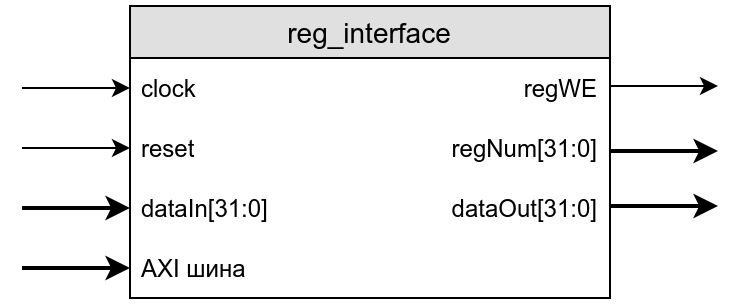
\includegraphics[width=0.5\linewidth]{reg_interface.png}
    \caption{Сигналы блока reg\_interface}
    \label{fig:reg_interface}
\end{figure}
Каждый пользовательский сигнал (\texttt{dataPLtoPS}, \texttt{regWE}, \texttt{regNum}, \texttt{dataPStoPL}) ассоциирован с определённым участком в памяти, таким образом, текущее значение по выбранному адресу является состоянием сигнала. Блок связан с модулем \texttt{reg\_file} программируемой логики, подробное описание которого будет приведено в соответствующей главе. Сейчас важно то, что этот модуль содержит виртуальные регистры, операции с ними осуществляются посредством рассматриваемого модуля \texttt{reg\_interface}, который переводит их в операции с реально существующими регистрами.\par
Для записи в виртуальный регистр необходимо вставить данные в сигнал \texttt{dataPStoPL}, затем установить номер регистра в сигнал \texttt{regNum}, после чего подать единицу в сигнал \texttt{regWE}.\par
Для чтения из виртуального регистра необходимо установить номер интересующего регистра в сигнал \texttt{regNum}, после считать данные из сигнала \texttt{dataPLtoPS}.\par
Общая диаграмма блоков процессорной системы изображена на рисунке \ref{fig:ps_top}.\par
\begin{figure}[ht]
    \centering
    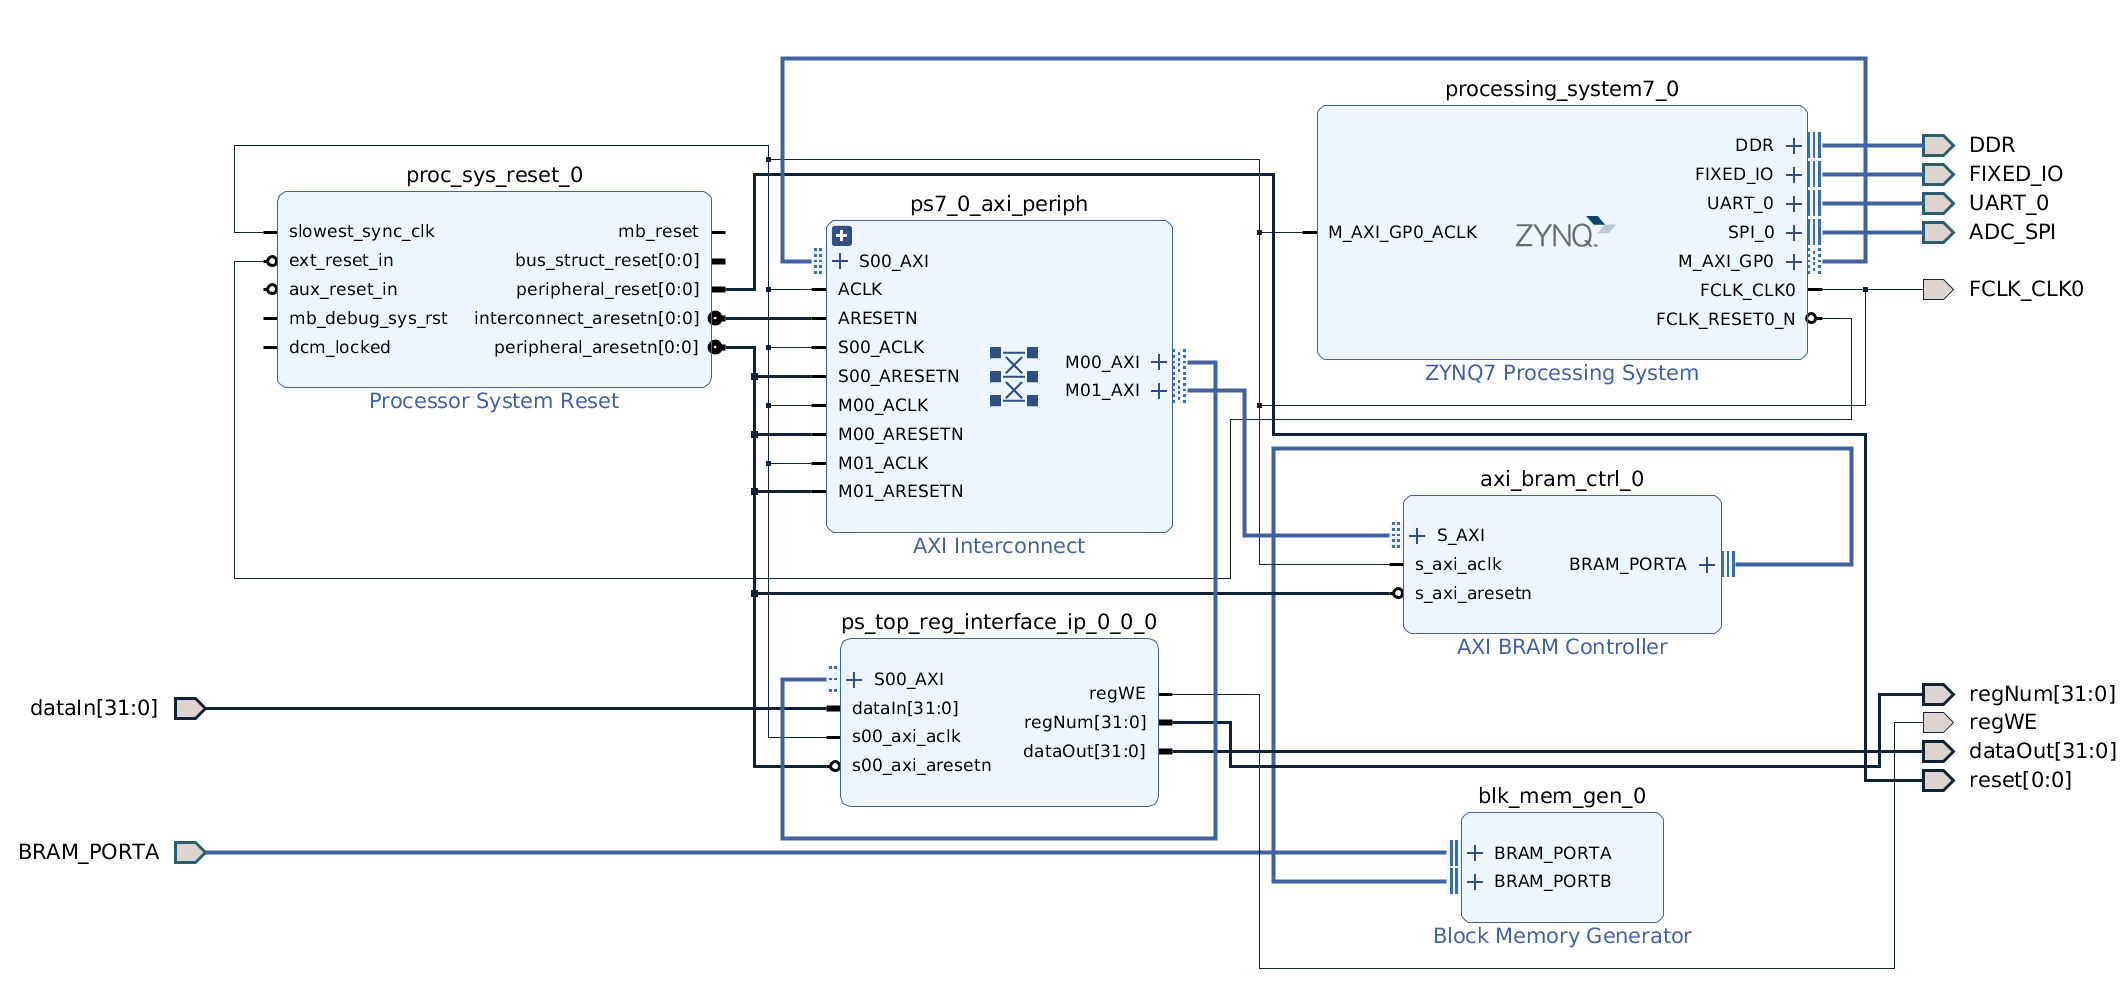
\includegraphics[width=1\linewidth]{ps_top.jpg}
    \caption{Диаграмма блоков процессорной системы}
    \label{fig:ps_top}
\end{figure}
Кроме интерфейса виртуальных регистров, рассмотренного выше, для обмена данными между процессорной системой и программируемой логикой используется модуль двухпортовой памяти \texttt{blk\_mem\_gen\_0}: через порт A происходит запись данных из программируемой логики, а через порт B информация считывается и отправляется в процессор. Настоящий модуль предназначен для передачи данных осциллограмм для их последующего отображения оператору стенда. Схожий блок двухпортовой памяти, необходимый для передачи статистических данных гистограмм расположен в части программируемой логики. Для их интеграции с интерфейсом шины AXI в процессорной системе предусмотрены контроллеры блоков памяти \texttt{oscillograms\_bram\_ctrl} и \texttt{spectra\_bram\_ctrl} соответственно.\par

